\begin{frame}{Bezier points calculation}
\begin{columns}[c] % The "c" option specifies centered vertical alignment while the "t" option is used for top vertical alignment

	\column{.45\textwidth} % Left column and width
	\vspace{5mm}
	\begin{figure}
	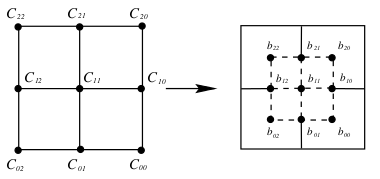
\includegraphics[width=\linewidth]{Pictures/BackupSlidesFitting/bezierPoints.png}
	\caption{from [3]}
	\end{figure}

	\column{.45\textwidth} % Right column and width
	\vspace{-3mm}
	\begin{equation*}
	\begin{array}{lcl} 
	b_{00} & = & (C_{00} + C_{10} + C_{01} + C_{11})/4 \\ 
	b_{10} & = & (C_{11} + C_{10})/2 \\
	b_{01} & = & (C_{11} + C_{01})/2 \\
	b_{11} & = & C_{11}
	\end{array}
	\end{equation*}
	\end{columns}

\end{frame}